%2011.4.4 ヤマサキ この章は大きく変更した箇所はありません。
\chapter{熱力学入門}

熱力学は「化学I」や秋学期「物理学II」で学ぶ。しかし, 
それらは力学と多くの接点を持つので, ここで概略を学んでおこう。

\section{温度の定義}

物質や物体は, 膨大な数の原子や分子から構成される。
それらの粒子どうしは引力や斥力を及ぼしあい, 時には衝突しつつ
共存する。その様子を知るには, 原理的には全粒子のそれぞれに
ついて運動方程式を解いて追跡すればよい。そのように個々の
粒子の挙動に注目する観点を\underline{微視的}(ミクロ)な観点という。

しかし, 現実的にはそれは大変だし, そこまでのくわしい様子を知る
必要も少ない。むしろ, 興味があるのは, 粒子集団が, 全体として, 
平均的にどのような性質を持つか, ということだ。そのような
観点を\underline{巨視的}(マクロ)な観点という。

熱力学は, 物質や物体の巨視的な性質を検討する。そのときに最初に
便利な指標が\underline{温度}だ\index{おんど@温度}。温度とは何だろう?
温度には様々な定義があるが, わかりやすいのは以下である
\footnote{ここで温度を$T$と表すことに注意。これまでは$T$は
運動エネルギーを表していたが, 慣習的には温度を表す方が多い。
そこで, この章では運動エネルギーは$T$ではなく$K$で表す。}:

\begin{itembox}{絶対温度の定義 (エネルギー等分配則とも言う)}\label{def:temperature0}
物体を構成する粒子について, ひとつの粒子・ひとつの自由度における
平均的な運動エネルギー$K$が
\begin{eqnarray}K=\frac{1}{2}\,k_{\text{B}}T\label{eq:def_temperature0}\end{eqnarray}
と書けるとき, $T$をその物体の絶対温度と呼ぶ。
$k_{\text{B}}$は\underline{ボルツマン定数}\index{ぼるつまんていすう@ボルツマン定数}と呼ばれる定数で, 
\begin{eqnarray}
k_{\text{B}}=1.38065...\times10^{-23}\text{ J K}^{-1}\label{eq:def_Bolconst}
\end{eqnarray}
\end{itembox}
\eref{eq:def_temperature0}, \eref{eq:def_Bolconst}をもとに定義される温度の単位を, K(ケルビン)
という\footnote{温度の単位を表すKの記号は, 他の単位の記号と同じように, 
立体(正体)である。それに対して, \eref{eq:def_temperature0}の左辺に
出てくる, 運動エネルギーを表す変数$K$は, 斜体で書いていることに注意。これらは全く
別物だ。}。

ここで\underline{自由度}\index{じゆうど@自由度}とは, 独立した
「運動の仕方」の数である。例えば単原子分子からなる気体(図\ref{fig:deg_freedom1})では, 
ひとつの分子(=原子)は3つの各方向($x$方向, $y$方向, $z$方向)に
自由に直線運動ができ, 各方向の運動は互いに独立である($x$方向に
大きな速度で飛ぶからといって$y$方向にはゆっくり飛ばねばならない, というような
制約は存在しない)。従って, 自由度は3である。

\begin{figure}[h]
    \centering
    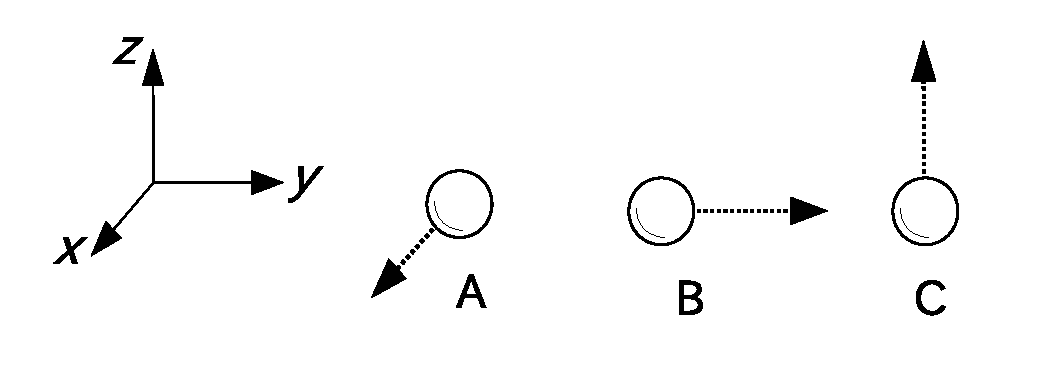
\includegraphics[width=8cm]{deg_freedom1.eps}
    \caption{単原子分子気体の自由度。A: $x$方向の直線運動, B: $y$方向の直線運動, C: $z$方向の直線運動。}\label{fig:deg_freedom1}
\end{figure}

\eref{eq:def_temperature0}は, 粒子の運動エネルギーが, 平均的には, 各自由度
に等しく割り当てられることも主張している。例えば, ある物質の中で, 多くの
粒子が同じ特定の方向にだけ激しく運動して, その方向の自由度だけに大きな運動エネルギー
を持つ, というような「偏った状態」にはならない, ということだ\footnote{それには
ちゃんとした理由があるのだが, 難しいのでここでは述べない。
興味ある人は, 「統計力学」という分野を勉強してみよう!}。その事情を表して, 
\eref{eq:def_temperature0}のことを\underline{エネルギー等分配則}
\index{えねるぎーとうぶんぱいそく@エネルギー等分配則}と呼ぶこともある。\mv

\eref{eq:def_temperature0}は「温度の定義」なので, とりあえずその由来や
正当性に疑問を持つ必要はない。むしろ不思議なのは, 
\eref{eq:def_temperature0}のように定義される温度が, 我々の感覚である
熱さ・冷たさや, 温度計の指す値にきちんと対応していることだ。そのあたり
は化学や物理学IIなどで学んでもらうとしよう。

\eref{eq:def_temperature0}は, 粒子の平均的な運動エネルギーは物体の
温度に比例することを主張している。その比例係数に「ボルツマン定数」という怪しげな
数とか「1/2」とかが現れているが, これらは「ケルビン」という「温度の単位」を人類が
採用してしまったことに対応するつじつま合わせ(単位換算)のための数に過ぎない。実際, 
運動エネルギーと温度が比例するのなら, いっそ(粒子の1自由度あたりの平均的な)
運動エネルギーそのものを温度としてしまえばよかったのだが, 今さらそれもめんどくさい
ので, 人類はこれからも, 温度とエネルギーを別の次元の物理量として扱っていくのだろう。\mv

\begin{q}\label{q:def_temperature}
絶対温度の定義を5回書いて記憶せよ。\end{q}\mv

\begin{q}\label{q:velocity_temperature}
質量$m$の気体分子の運動を考える。各分子が速度$(v_x, v_y, v_z)$で空間を飛ぶとき, 
エネルギー等分配則によって, $v_x$に関する運動エネルギー, つまり$mv_x^2/2$の平均は, $k_{\text{B}}T/2$
となる。従って, 平均的には\footnote{厳密には, $v_x$の二乗平均平方根(root-mean-square)。}
\begin{eqnarray}|v_x|=\sqrt{\frac{k_{\text{B}}T}{m}}\label{eq:velocity_temperature1}\end{eqnarray}
となる。$|v_y|$, $|v_z|$についても同様である。すると, 速度の大きさ(つまり速さ)$v$は, 
\begin{eqnarray}v=\sqrt{v_x^2+v_y^2+v_z^2}\label{eq:velocity_temperature2}\end{eqnarray}
なので, $v$は平均的には, 
\begin{eqnarray}v=\sqrt{3\frac{k_{\text{B}}T}{m}}\label{eq:velocity_temperature3}\end{eqnarray}
となる。以下, $T=300$ K(摂氏27度)で考える:
\begin{enumerate}
\item 水素分子H$_2$の$x$方向の平均的な速さを求めよ。
\item 水素分子H$_2$の平均的な速さを求めよ。
\item 窒素分子N$_2$の平均的な速さを求めよ。
\end{enumerate}
\end{q}

ところで, 「化学」で, 「グラハムの法則」\index{ぐらはむのほうそく@グラハムの法則}
というのを習った人もいるだろう。それは, 気体分子の速さ$v$が, 
その質量$m$の平方根に反比例する, という
法則だ。これは, \eref{eq:velocity_temperature3}で明らかだ。
\vspace{0.6cm}


\section{理想気体の状態方程式 (気体分子運動論)}

これまで学んだことを使って, 気体の温度・圧力・体積の間の関係を理論的に導いてみよう。

今, 簡単のため, 一辺の長さが$L$の立方体の箱を考える。
図\ref{fig:gas_motion}のように, 立方体の中心を原点Oとし, 
$x$, $y$, $z$軸のそれぞれに立方体の面が直交するように座標軸を設定する。
点$(L/2, 0, 0)$で$x$軸と直交する面を面Aと呼ぶ。
\begin{figure}[h]
    \centering
    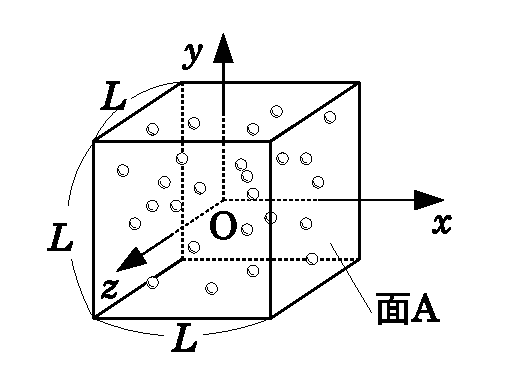
\includegraphics[width=8cm]{gas_motion.eps}
    \caption{気体分子の運動を考える座標系と箱。}\label{fig:gas_motion}
\end{figure}

この箱の中に, $N$個の気体分子が入っているとする。ここで, 以下の仮定を置く:
\begin{itembox}{理想気体の仮定}
\begin{itemize}
\item 気体分子の大きさは十分に小さい。
\item 気体分子同士に働く力は無視できる。
\end{itemize}
\end{itembox}
この2つの仮定を満たす分子からなる気体を「理想気体」という。
今, 立方体の中には理想気体が入っているとする。

箱の内側では気体分子が飛び交っており, 絶えずその一部が面Aに内側から衝突し, 
跳ね返されている。この衝撃が, 面Aを外に押し出そうとする。従って, それを打ち
消すように, 外側から適当な圧力($P$とする)をかけないと, この箱は壊れて
しまうだろう(図\ref{fig:gas_motionA})。

\begin{figure}[h]
    \centering
    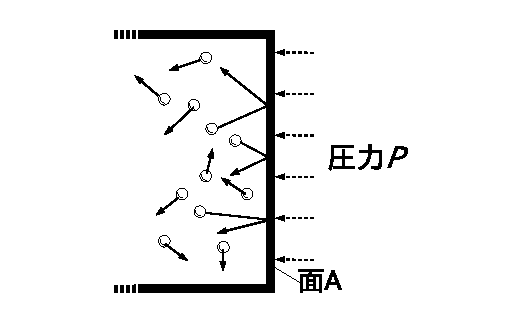
\includegraphics[width=8cm]{gas_motionA.eps}
    \caption{面Aの付近 ($z$軸の正の方向から見たところ)。分子が面Aにひっきりなしに
ぶつかるので, 面Aを外側から圧力$P$で支えていないといけない。}\label{fig:gas_motionA}
\end{figure}

その事情を詳しく見てみよう: 今, 簡単のために, どの気体分子も, $x$軸に沿った方向($x$軸の
正の方向か負の方向)に一定値$|v_x|$という速さで動いているとしよう。つまり, $x$軸方向の
速度は, $|v_x|$か$-|v_x|$であるとする(実際は気体分子の速度はもっといろんな可能性があり, 
$x$軸に沿った速度の二乗平均平方根が$|v_x|$に等しいだけだが, 仮にそういうのを考慮して厳密に理論展開
しても, 以下と同じ結論に至る)。従って, どの気体分子も, 時間$\Delta t$の間に, 
$|v_x| \Delta t$だけ$x$軸に沿って移動する。従って, 時間$\Delta t$の間に, 内側から面Aに
衝突する気体分子は, 面Aから距離$v_x \Delta t$までの領域にいるはずだ。その領域の体積は
\begin{eqnarray}L^2v_x\Delta t\label{eq:gas_stat_eq_0}\end{eqnarray}
である。箱の中の気体分子は均等に分布すると考えれば, 上述の領域の中の分子数は, 
領域の体積に比例するので, 
\begin{eqnarray}\frac{L^2v_x\Delta t}{L^3}N\label{eq:gas_stat_eq_1}\end{eqnarray}
となる\footnote{箱の体積は$L^3$であり, その中に$N$個の気体分子が均等に分布している。
従って, 箱の中の気体分子の数密度(単位体積当たりの分子数)は, $N/L^3$だ。これに, 
いま考えている領域の体積(\eref{eq:gas_stat_eq_0})をかければ, その領域内の気体分子数
が得られるはずだ。それが\eref{eq:gas_stat_eq_1}である。}。この個数のうち, 
半分が$x$軸の正方向, 半分が$x$軸の負の方向に進むので, 面Aに衝突する個数は, 
\begin{eqnarray}
\frac{1}{2}\frac{L^2v_x\Delta t}{L^3}N=\frac{Nv_x\Delta t}{2L}\label{fig:gas_motion_hitnum}
\end{eqnarray}
となる。

さて, 気体分子1個が面Aにぶつかって跳ね返る状況を考えよう。気体分子が跳ね返る時, 
面Aとの間に摩擦が働かず, 分子の運動エネルギーは変化しない(弾性衝突)とすると, 
面Aに平行な速度成分 ($v_y$と$v_z$) は変化せず, 面Aに垂直な成分($v_x$)が, 
大きさを変えずに符号だけ反転する。すると, $x$方向の運動量は, 
衝突前は$mv_x$, 衝突後は$-mv_x$になるので, 結局, 1個の気体分子の
衝突前後の運動量変化は次式になる:
\begin{eqnarray}
-mv_x-(mv_x)=-2mv_x\label{fig:gas_motion_changemom}
\end{eqnarray}

実際は1個でなく, \eref{fig:gas_motion_hitnum}で表される個数が$\Delta t$の
間に面Aにぶつかるので, それらの運動量変化の合計は次式になる:
\begin{eqnarray}
\frac{Nv_x\Delta t}{2L}\times(-2mv_x)=-\frac{Nmv_x^2\Delta t}{L}\label{eq:gas_motion_collide}
\end{eqnarray}
この運動量変化は, 面Aに外側からかかる力がもたらす力積に等しい
はずだ(運動量変化=加えられた力積)。

面にかかる力は, 圧力×面積であり, 面Aの面積は$L^2$だ。
従って, 面Aに(外側から)かかる力は$-PL^2$である(マイナスは, 力の向き, 
つまり$x$軸の負の方向を表すためにつけた)。その力による力積は, 
\begin{eqnarray}-PL^2\Delta t\label{eq:gas_motion_collide2}\end{eqnarray}
となる。\eref{eq:gas_motion_collide}と\eref{eq:gas_motion_collide2}が
一致することが, 面Aが静止する条件である:
\begin{eqnarray}-PL^2\Delta t=-\frac{Nmv_x^2\Delta t}{L}\end{eqnarray}
これを整理すると, 
\begin{eqnarray}PL^3=Nmv_x^2\label{eq:gas_stat_eq_5}\end{eqnarray}
となる。いま, $L^3$は箱の体積$V$なので, \eref{eq:gas_stat_eq_5}は
\begin{eqnarray}PV=Nmv_x^2\label{eq:gas_stat_eq_6}\end{eqnarray}
となる。さらに, \eref{eq:velocity_temperature1}より, 
\begin{eqnarray}v_x^2=\frac{k_{\text{B}}T}{m}\end{eqnarray}
なので, \eref{eq:gas_stat_eq_6}は, 以下のようになる:
\begin{itembox}{理想気体の状態方程式}
\begin{eqnarray}PV=Nk_{\text{B}}T\label{eq:gas_stat_eq_7}\end{eqnarray}
\end{itembox}

ここで, 分子数を「個」でなくて「モル」で数えよう。すなわち, $N$個が$n$モルに相当
するとすれば, $N=nN_\text{A}$である($N_\text{A}$はアボガドロ定数)。従って, \eref{eq:gas_stat_eq_7}は, 
\begin{eqnarray}PV=nN_\text{A}k_{\text{B}}T\label{eq:gas_stat_eq_72}\end{eqnarray}
となる。ここで, 物理学の慣習として, 以下の定数を導入する:
\begin{itembox}{気体定数の定義}
以下で定義される定数$R$を, 気体定数(gas constant)と呼ぶ:
\begin{eqnarray}R=N_\text{A}k_{\text{B}}\label{eq:def_gas_const}\end{eqnarray}
その値は, 8.314472... J~mol$^{-1}$K$^{-1}$である。
\end{itembox}
すると, \eref{eq:gas_stat_eq_72}は, 以下のように書ける:
\begin{itembox}{理想気体の状態方程式(モルで表す場合)}
\begin{eqnarray}PV=nRT\label{eq:gas_stat_eq_74}\end{eqnarray}
\end{itembox}

\begin{q}\label{q:def_ideal_gas}
理想気体とは何か?
\end{q}\mv

\begin{q}\label{q:ideal_gas_eq}
理想気体の状態方程式を導出せよ(上記の解説を整理して再現すればよい)。
\end{q}\mv

\begin{q}\label{q:tempera_kBR} 
\begin{enumerate}
\item ボルツマン定数$k_{\text B}$の値を, 有効数字3桁で述べよ。
\item 気体定数$R$の値を, 有効数字3桁で述べよ。
\item ボルツマン定数と気体定数の関係を, 式で述べよ。
\end{enumerate}\end{q}
\hv



\section{理想気体の内部エネルギーと温度}

さて, 物質や物体を構成する全ての粒子のエネルギー(運動エネルギーとポテンシャルエネルギー)を
合計したものを, その物質や物体の「内部エネルギー」という(定義)。ここで, 理想気体を考えよう。 
理想気体では, 気体分子が相互に及ぼす力は無視できるので, 気体分子同士が及ぼし合う力による
ポテンシャルエネルギーは無視してもかまわない。また, 非常な低温でもない限り, 重力による
ポテンシャルエネルギーは, 運動エネルギーよりはるかに小さい。従って, 
理想気体の内部エネルギーは, 大部分が構成粒子(気体分子)の運動エネルギーの総和であると
考えてよい\footnote{もし粒子が電離していたら, 電気的なポテンシャルエネルギーを持つ
かもしれないが, その場合は粒子同士の間にクーロン力が働くので, 理想気体の仮定に反する。
従って, 電気的なポテンシャルエネルギーも考えなくてよい。}。

エネルギー等分配則によれば, 運動エネルギーは1粒子あたり・1自由度あたり, 
平均的に$k_{\text{B}}T/2$だ。すると, 自由度$F$を持つ気体分子が$N$個からなる気体の内部エネルギー$U$
は\footnote{力学では, $U$は多くの場合, ポテンシャルエネルギーを表す記号として慣習的に使われる。
しかし, 熱力学では慣習的に$U$は内部エネルギーを表す。ここでは熱力学の慣習に従う。}, 
\begin{eqnarray}U=\frac{F}{2}Nk_{\text{B}}T\label{eq:gas_int_energy0}\end{eqnarray}
となる。すなわち, \underline{理想気体の内部エネルギーは}, \underline{温度に比例し, 
圧力や体積とは直接には無関係である}\footnote{もちろん, 圧力と体積は温度と関係があるから, 
圧力や体積は, 温度を介して間接的な関係はある。}。

さて, \eref{eq:gas_int_energy0}において分子が$n$モルあるとすると, $N=nN_{\text A}$だから, 
\begin{eqnarray}U=\frac{F}{2}nN_{\text A}k_{\text B}T\end{eqnarray}
となる。\eref{eq:def_gas_const}を使うと, 
\begin{eqnarray}U=\frac{F}{2}nRT\label{eq:gas_int_energy1}\end{eqnarray}
となる。特に, 分子数を1モルとすると, 
\begin{eqnarray}U=\frac{F}{2}RT\label{eq:gas_int_energy3}\end{eqnarray}
となる。

では, 自由度$F$はどう決まるのだろうか? 前述のように, 単原子分子気体(He, Ne等)は
3方向の直線運動の自由度を持つので$F=3$である。ところが, 2原子分子(H$_2$, O$_2$, N$_2$等)は
直線運動だけでなく, 回転運動も行う\footnote{回転運動にも運動エネルギーが
与えられることは, 後の章で学ぶ。}。直線状の棒を回すのには独立した(つまり互いに直交した)
軸が2つある\footnote{一般に, 物体を回転させる独立な回転軸は3つある。しかし, 
直線状の分子の場合は, 直線の断面は大きさを持たない点とみなしてよい。従って, 
直線を軸にする回転は考えなくてよい。同様に, 1原子分子は点とみなしてよいので, 
いずれの方向を軸とする回転も, 考えなくてよい。}ので, これらの回転の自由度は2である。
従って, これらの分子の自由度$F$は, 直線運動に3, 回転運動に2で, 合計5となる(図\ref{fig:deg_freedom2})。

\begin{figure}[h]
    \centering
    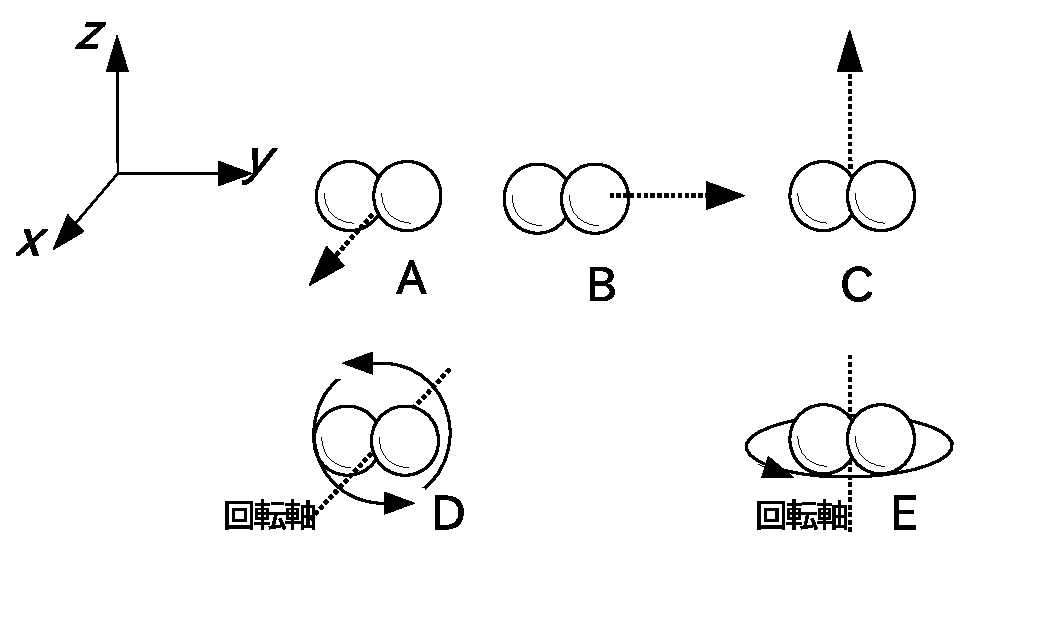
\includegraphics[width=8cm]{deg_freedom2.eps}
    \caption{2原子分子気体の自由度。A: $x$方向の直線運動, B: $y$方向の直線運動, C: $z$方向の直線運動, D: $x$軸まわりの回転運動, E: $z$軸まわりの回転運動。}\label{fig:deg_freedom2}
\end{figure}

従って, 理想気体1モルあたりの内部エネルギーは, 

\begin{eqnarray}
\text{単原子分子理想気体では, }U&=&\frac{3}{2}RT\label{eq:U_monomol}\\
\text{2原子分子理想気体では, }U&=&\frac{5}{2}RT\label{eq:U_2mol}
\end{eqnarray}
となる\footnote{高校で化学や物理学を学んだ人は, これは
「定積モル比熱」と「定圧モル比熱」の話か, と思うかもしれないが, そうではない。
その話はこの後に出てくる。}。

このように, 同じ温度, 同じモル数であっても, 分子が単原子分子か, 2原子分子かによって, 
内部エネルギーは違うのである。分子が複雑な運動をする可能性があるほど(つまり自由度が
大きいほど), 気体は大きな内部エネルギーを持つのである。
\footnote{理想気体では分子の大きさは無視できるはずなのに, 「2原子」分子を考える
のは変ではないか, と思う人もいるかもしれない。実は, 理想気体で「分子の大きさを無視する」
としたのは, 分子の大きさによって容器(分子が自由に飛び交うことのできる空間)の体積
が実質的に目減りするようなことがない, という意味だ。それに対して, 2原子分子を
考えるのは, 分子の回転運動が運動エネルギーを持つという性質を勘案するためであり, 
それは理想気体の仮定とは無関係である。}。

ただし, これらの式は(たとえ理想気体に対しても)厳密には成り立たない。特に, 低温になると, 
回転の自由度が意味を持たなくなる(自由度が減る)とか, 高温になると振動の自由度が
加わってくる(自由度が増える)などの, 不思議な現象が起きる。それらは量子力学を使わないと説明できない。\\



\section{比熱と熱容量}

ここで, 「熱容量」\index{ねつようりょう@熱容量}と「比熱」\index{ひねつ@比熱}
という概念を学ぼう。

ある物体の熱容量とは, その物体の温度を単位温度だけ上げるのに必要な熱量
のことである。すなわち, ある物体に熱量$dQ$を加えた時の温度の変化が
$dT$のとき, $dQ/dT$のことを熱容量と呼ぶ(定義)。熱容量は温度によって
変わることがあるので, この$dQ$や$dT$は, できるだけ小さい値(微小量)であるべきである。

単位量の物質の熱容量を「比熱」という。すなわち, ある物体の物質量が$X$であり, 
その物質に熱量$dQ$を加えた時の温度の変化が$dT$のとき, $dQ/(X\,dT)$の
ことを比熱と呼ぶ(定義)。特に, 物質量$X$を質量で表すときに「比熱」と呼び, 
物質量$X$をモルで表すときには「モル比熱」と呼ぶ。

熱容量は「物体」に関する量であり, 比熱は「物質」に関する量である。\\


\section{理想気体の定積モル比熱}

では, 理想気体の比熱について学ぼう。ここではモル比熱を考える。

気体に熱を加えたら, 普通, 気体はあたたまるだろう。しかし, 同時に, 気体は
膨張もする。このとき, 問\ref{q:gas_work}で見たように, 気体は仕事をする。
その仕事のぶんだけ, どこかからエネルギーが必要である(エネルギー保存則!)。
それは, 気体に加えられた熱かもしれないし, 気体がもともと持っていた内部エネルギー
かもしれない。

とりあえずそういう面倒なことを考えるのは避けたいので, 温めても気体は膨張しない
条件, すなわち気体をガッチリした容器に入れて体積が変わらないようにして温める
ことを考えよう。このように体積一定での変化を定積変化とか定積過程と呼ぶ。
定積変化でのモル比熱を「定積モル比熱」\index{ていせきもるひねつ@定積モル比熱}
と呼び, $C_{\text{v}}$と書く(添字のvは, volumeのv。volumeが変わらないよ, 
という意味)。

体積が変わらないなら, 加えた熱は全部内部エネルギーに変わる。$n$モルの理想気体の
内部エネルギー$U$は, \eref{eq:gas_int_energy1}より, 
\begin{eqnarray}
U=\frac{F}{2}nRT\label{eq:specific_heat_vconst2}
\end{eqnarray}
である。ここで熱量$dQ$を加えて温度が$dT$だけ上がったとすると, 内部エネルギーは$U+dQ$, 
温度は$T+dT$になるから, 
\begin{eqnarray}
U+dQ=\frac{F}{2}nR(T+dT)\label{eq:specific_heat_vconst4}
\end{eqnarray}
である。\eref{eq:specific_heat_vconst4}から\eref{eq:specific_heat_vconst2}を
辺々引くと, 
\begin{eqnarray}
dQ=\frac{F}{2}nR\,dT\label{eq:specific_heat_vconst6}
\end{eqnarray}
となる。従って, 定積モル比熱は, 
\begin{eqnarray}
C_{\text{v}}=\frac{dQ}{n\,dT}=\frac{F}{2}R\label{eq:gas_specificheat}
\end{eqnarray}
となる。特に, 
\begin{eqnarray}
\text{単原子分子理想気体では, }C_{\text{v}}&=&\frac{3}{2}R\label{eq:Cv_monomol}\\
\text{2原子分子理想気体では, }C_{\text{v}}&=&\frac{5}{2}R\label{eq:Cv_2mol}
\end{eqnarray}
である。そして, \eref{eq:gas_specificheat}と\eref{eq:gas_int_energy1}を見比べれば, 
\begin{eqnarray}
U=n\,C_{\text{v}}\,T\label{eq:U_nCvT}
\end{eqnarray}
であることがわかる。この式は, 明らかに, 定積変化という条件とは
無関係に成り立つ。つまり, 理想気体の内部エネルギーは, 一般的に, モル数と
定積モル比熱と絶対温度の積である。

では, 「体積一定」という条件を外したら, 理想気体のモル比熱はどうなるだろうか?
それを検討するには, 気体の内部エネルギーと熱と仕事について, ここで
しっかり考え方を固めておかねばならない。それが次節の内容である。\\



\section{熱力学第一法則}

我々は既に「力学的エネルギー保存則」を学んだが, エネルギーは, 
熱も含めて, より広い範囲で保存する(どこかに消えたりどこかから
湧いて出たりしない)。そのことを熱力学でも利用する。それは以下のような
形である:
\begin{eqnarray}
\Delta U=Q+W\label{eq:thermlaw1}
\end{eqnarray}
ただし, $U$は系の内部エネルギー, $\Delta U$は内部エネルギーの
変化, $Q$は外から系に与えられた熱, $W$は外から系になされた
仕事である。要するに「熱と仕事が与えられたぶんだけエネルギーが増える」
というわけだ。

\begin{q}\label{q:themlaw1} 熱力学第一法則を5回書いて記憶せよ。
「ただし書き」もちゃんと書くこと!\end{q}\mv

ここで, $\Delta U$は微小量でなくても構わない。普通, $\Delta$なんちゃら
というと, (有限な)微小量を考えることが多いが, 熱力学で出てくる
$\Delta$は「微小」ではない, 単なる「差」とか「変化」を表す。
微小を意味するときは, $\Delta$でなく$d$を使うことが多い。
微小量で\eref{eq:thermlaw1}を表現すると, 
\begin{eqnarray}
dU=dQ+dW\label{eq:thermlaw1inf}
\end{eqnarray}
となる($dQ$は外から系に加えられた微小な熱, $dW$は外から系になされた
微小な仕事)。ところが, \eref{eq:gas_work5}で学んだように, 気体の体積の微小な
変化$dV$に伴って, 系が外界からされる仕事は, 
\begin{eqnarray}dW=-P\,dV\end{eqnarray}
である。これを使うと上の式は, 
\begin{eqnarray}
dU=dQ-P\,dV\label{/eq:thermlaw1infPdV}
\end{eqnarray}
と書ける。これを変形すると, 次式になる: 
\begin{eqnarray}
dU+P\,dV=dQ\label{eq:thermlaw1infPdV2}
\end{eqnarray}
これは微小量での式だが, \textgt{もし圧力$P$が一定ならば}, 容易に
積分できて, 
\begin{eqnarray}
\Delta U+P\Delta V=Q\label{eq:thermlaw1infPdV3}
\end{eqnarray}
となる。


\section{理想気体の定圧モル比熱}

では, 「体積一定」という条件を外して, 理想気体のモル比熱を考えよう。
といっても, ここでは特に, 「圧力一定」という条件で考えよう。そのような条件での変化を
「定圧変化」とか「定圧過程」という。定圧過程でのモル比熱を「定圧モル比熱」
と呼び, $C_{\text{p}}$と表す。

$C_{\text{p}}$を求めるには, 熱力学第一法則から出発する。ここでは
\eref{eq:thermlaw1infPdV2}から出発しよう。この式の左右を入れ替え, 
\eref{eq:U_nCvT}を使えば, 
\begin{eqnarray}
dQ=nC_{\text{v}}dT+P\,dV
\end{eqnarray}
である。

ところで, 理想気体の状態方程式から, $PV=nRT$である。$P$と$n$は一定であり, 
$R$は定数なので, $P\,dV=nR\,dT$である。これを上の式に代入すれば, 
\begin{eqnarray}
dQ=nC_{\text{v}}dT+nR\,dT=n(C_{\text{v}}+R)\,dT
\end{eqnarray}
となる。従って, 
\begin{eqnarray}
C_{\text{p}}=\frac{dQ}{n\,dT}=C_{\text{v}}+R
\end{eqnarray}
である。つまり, 定圧モル比熱は, 定積モル比熱に気体定数を加えたものである。

\begin{q} 以下を示せ:
\begin{eqnarray}
\text{単原子分子理想気体では, }C_{\text{p}}&=&\frac{5}{2}R\label{eq:Cp_monomol}\\
\text{2原子分子理想気体では, }C_{\text{p}}&=&\frac{7}{2}R\label{eq:Cp_2mol}
\end{eqnarray}
\end{q}

\begin{faq}{\small\textgt{\eref{eq:thermlaw1infPdV3}が
ピンと来ません。「加えられた熱」$Q$が「内部エネルギーの変化」$\Delta U$に
等しいのはわかります。でも, 仕事$P\Delta V$というのがわかりません}
 ... では例を挙げましょう。純粋なエタノール(液体)と純水(液体)をまぜると, 
できた「エタノール水溶液」は暖かくなります(やったことがなければやってみて
ください!)。この熱はどこから来るのでしょう? エタノール分子は水分子と
引き合いますから, それらどうしがくっつくと(水和すると), 互いの引力
のポテンシャルエネルギーが, 熱として放出されるのです。これが
$\Delta U$にあたります。ここでは$U$は小さくなるので, $\Delta U$は
マイナスです。つまり, 系に熱を「加える」のではなく系から熱が「出る」のです。
だから温かくなるのです。

しかし! それだけではないのです! エタノール水溶液の体積は, 
元のエタノールの体積と水の体積を足したものよりも, わずかに小さく
なります。縮むのです! このとき, 体積が縮む分, 周囲の大気は水溶液
に対して仕事をします。それが$P\Delta V$です。ここでは$\Delta V$は
マイナスですので, $P\Delta V$もマイナスです。つまり, その仕事も
外に熱として出るのです。

従って, 水溶液が温かくなるのは, 分子同士の引力によるポテンシャルエネルギー
と, 水溶液の体積が小さくなることに伴う外部(大気)による仕事の両方
が寄与するのです。

このように, 反応熱を考えるには, 単に分子同士の引力や斥力だけでなく, 
まわりの環境からの仕事も考慮する必要があります。それをうまく整理して
くれるのが, 次節の「エンタルピー」です。}\end{faq}\mv


\section{エンタルピー}

生物資源学類では, 1年次「化学I」で, エンタルピーという概念を習う。
エンタルピーは, 化学反応や相変化を予測したり制御するのに必要な
概念であり, 特に, 「反応熱」に関わっている。

ところが, 多くの1年生は「エンタルピーって結局何?」と悩む。おまけに, 
そのあとに「エントロピー」という紛らわしい概念が出てきて混乱する。

\textgt{そのような悩みは, 定義を覚えていないことから発する}。
くどいようだが, まず定義をきちんと覚えないと何も話がはじまらない。
\begin{itembox}{エンタルピーの定義}
系の内部エネルギーを$U$, 圧力を$P$, 体積を$V$とすると, 
\begin{eqnarray}
H:=U+PV\label{eq:def_enthalpy}
\end{eqnarray}
をエンタルピーという(定義)。
\end{itembox}

\begin{q}\label{q:def_enthalpy} エンタルピーの定義を5回書いて記憶せよ。\end{q}\mv

さて, 定義を覚えたら, エンタルピーの意味を少しずつ考えていこう。
まず, この$H$の変化を考えてみよう。すなわち, ある状態(内部エネルギー
$U$, 圧力$P$, 体積$V$, エンタルピー$H$)から変化した状態
(内部エネルギー$U+\Delta U$, 圧力$P+\Delta P$, 体積$V+\Delta V$, エンタルピー$H+\Delta H$)
を考え, そのときのエンタルピーの変化を考えよう。変化前は, 
\begin{eqnarray}
H=U+PV
\end{eqnarray}
変化後は, 
\begin{eqnarray}
H+\Delta H=(U+\Delta U)+(P+\Delta P)(V+\Delta V)\nonumber\\
\end{eqnarray}
後者から前者を引くと, 
\begin{eqnarray}
\Delta H=\Delta U+P\Delta V+V\Delta P+\Delta P\Delta V\label{eq:enthalpy_change05}
\end{eqnarray}
となる。\textgt{もしこの変化が, 圧力は不変(一定)の状態で
行われたら}, $\Delta P=0$なので, 上の式は, 
\begin{eqnarray}
\Delta H=\Delta U+P\Delta V
\end{eqnarray}
となる。この右辺は\eref{eq:thermlaw1infPdV3}の左辺と同じだ。従って, 
\begin{eqnarray}
\Delta H=Q
\end{eqnarray}
となる。つまり, \textgt{定圧変化では, 系に加えられた熱量は, 
エンタルピーの変化(増加分)に等しい}。これがエンタルピーの「意味」だ。

\begin{faq}{\small\textgt{これがエンタルピーの意味だと言われても, 
ピンと来ません。なんで定圧に限定するのですか? それで何が嬉しいのですか? 
「系に加えられた熱量」がわかって何が嬉しいのですか?}
 ... まず, 世の中の現象の多く, 特に地上で起きる現象の多くは圧力
一定のもとで起きます。例えば君が料理を作る時, 圧力釜などを使わない
限り, 煮る・焼く・蒸す・混ぜる・凍らす・解凍するなどは, 一定の圧力(大気圧)
のもとで起きます。従って, 定圧を仮定しても, 理論の適用範囲はそんなには
限定されません。むしろ, 定圧を仮定することで, 現象の記述や解析は
単純になり, 楽になります。「系に加えられた熱量」は, 言葉を変えれば, 
「その変化を起こすのに外から加えねばならない必要な熱量」とも言えます。
また, これがマイナスの場合は, 「系から外に出る熱量」(要するに反応熱)
です。化学反応を制御したり, その反応熱を利用したりするとき, こういうのって, 
めっちゃ大事じゃないですか!}\end{faq}\mv


\section{エントロピー}

次に学ぶのは「エントロピー」である。エントロピーは, たくさんの分子や原子
からなる集団が, 全体としてどのように自発的にふるまうかを説明するときに
必要な概念である。

エントロピーはエンタルピーに名前が似ているので, 初学者は混同しやすいが, 
両者は全く異なる量である。名前が似ているのは偶然に過ぎない。そもそも名前が
似ているからといって、実体どうしも似ているとか互いに関係があるとはかぎらない。
例えば, 福井県の小浜市と米国元大統領のオバマ氏は名前が似ているが実体
は全く違う。エントロピーとエンタルピーもそういうものだと思っておけばよい。\\

まずエントロピーのその定義を述べよう。系には各状態において「エントロピー」
という量があり, 状態1のときのエントロピーを$S_1$, 状態2のときの
エントロピーを$S_2$とし, 
エントロピーの差, すなわち$S_2-S_1$を$\Delta S$とすれば, $\Delta S$は
次式を満たす, と約束する:
\begin{itembox}{エントロピーの定義1}
\begin{eqnarray}
\Delta S=\int_{\text{状態1}}^{\text{状態2}} \frac{dQ_{\text{rev}}}{T}\label{eq:def_entropy}
\end{eqnarray}
\end{itembox}
ここで, 積分は, 系が状態1から状態2まで\textgt{可逆的に}変化したときに
関するものであり, $Q_{\text{rev}}$は外から系に\textgt{可逆的に}
与えられる熱量, $T$は絶対温度である。 これがエントロピーの定義である。
「可逆的」の意味は次節で述べる。

もし, 状態1と状態2が互いに非常に近い状態であるとき, すなわち変化の量が微小
であるとき, $\Delta S$は微小量$dS$と書くことができ, また, 微小変化の間で
温度$T$はほとんど変わらないと考えてよいので, 上の式は, 
\begin{itembox}{エントロピーの定義2}
\begin{eqnarray}
dS=\frac{dQ_{\text{rev}}}{T}\label{eq:def_entropy2}
\end{eqnarray}
\end{itembox}
と書いてもよい。

このように, エントロピーは, それ自体ではなく, その「変化」が先に定義される。

と言われても, 「わかりにくい!」というのが正直なところだろう。そう, エントロピー
は初学者にはなかなかわかりにくいのだ。諸君はまず, \eref{eq:def_entropy}, \eref{eq:def_entropy2}
をしっかり頭に叩き込もう。そして, それをもとに, いろんな話について行けば, 
次第にエントロピーが何なのか, わかってくるだろう。
\hv

\begin{q}\label{q:def_enthalpy} 上のエントロピーの
定義をそれぞれ5回書いて記憶せよ。\end{q}\mv


\section{可逆過程}

以後, 少しずつ, エントロピーの「意味」を理解していこう。

まず, エントロピーの定義で, 「可逆的に」\index{かぎゃくてき@可逆的}という
言葉が出てきた。これはとても大切なキーワードである。

ある系の状態が変化したとき, (その気になれば)変化後の状態から変化前の
状態に戻すことができ, しかも外部に何の影響も残さないようにそれができる
場合, そのような変化を「可逆的な変化」あるいは「可逆過程」という(定義)。

\begin{exmpl}\label{exmpl:lift_reverse} 物体を重力に逆らってゆっくり持ち上げるというのは可逆過程である。
持ち上げるときにエネルギー(=仕事=重さ×持ち上げた高さ)が必要だが, 
持ち上がった後に, 物体を元の高さまで戻すならば, 重力が仕事をして, 
持ち上げた時に使ったエネルギーを埋め合わす。\end{exmpl}

\begin{exmpl} ある速さで地面を滑っていた物体が, 地面との摩擦によって止まる, 
というのは可逆過程ではない。というのも, 物体が持っていた運動エネルギー
は摩擦によって熱エネルギーに変えられてしまう。この変えられた熱エネルギー
をもういちど集めて, 物体の運動エネルギーに変えて, 物体を滑らせるという
のは, どう考えても無理である。\end{exmpl}

熱力学では, 気体の状態変化がよく例に使われるので, 以後はそういう話に
絞ろう。\\

まず, 外部に熱が出入りしないように気体を圧縮させたり膨張させたりする過程, 
すなわち\textgt{断熱過程は, 可逆過程である}。なぜか? 
変化に必要なのは外部との仕事のやりとりだけである。
仕事は例\ref{exmpl:lift_reverse}のようにたくわえたり放出したりできるので, 
元に戻すときに, 外部に何も影響を残さない。

断熱変化におけるエントロピー(の変化)は? そもそも外から系には出入りしないので, 
\eref{eq:def_entropy}の$dQ_{\text{rev}}$はゼロである。従って, この積分も0であり, 
従って, エントロピーの変化も0である。要するに, \textgt{理想気体の
断熱変化ではエントロピーは変化しない}。\\

また, 系の温度が変わらない変化(等温変化)はどうだろうか?

\begin{exmpl}\label{exmpl:gas_expand_rev} 
ある気体を, 温度を一定に保ったまま, 体積を膨張または圧縮させることを考える。
このとき, その気体をピストンに入れたまま, 同じ温度を持つ大きな環境
(熱容量が無限に大きなもの, たとえば大きなお風呂)に浸して変化させる
ものとしよう。ゆっくり気体を膨張させたとき, 気体は環境に対して仕事をするが, 
それに必要な仕事と同じだけの熱が, 環境から気体に流れ込む。逆に, 
気体をゆっくり圧縮したときは, 環境は気体に仕事をするが, その仕事と
同じだけの熱が, 気体から環境に流れ出す。このように, 変化を元に戻すときに, 
外部(環境)に何も影響を残さない。従って, \textgt{理想気体の等温変化は
可逆過程である}。

このときのエントロピー(の変化)はどうなるだろう? 
まず, 熱力学第一法則から, 熱の出入りを見積もろう。\eref{eq:thermlaw1infPdV2}より, 
\begin{eqnarray}
dU+P\,dV=dQ
\end{eqnarray}
である。理想気体の内部エネルギー$U$は温度だけに依存し, 圧力$P$や体積$V$には無関係
なので, 等温変化の前後では$U$は変わらない。従って, $P\,dV=dQ$である。等温変化は
可逆的なので$dQ$は$dQ_{\text{rev}}$であり, \eref{eq:def_entropy}より, 
\begin{eqnarray}
\Delta S=\int_{\text{状態1}}^{\text{状態2}} \frac{dQ_{\text{rev}}}{T}=\int_{V_1}^{V_2}\frac{P\,dV}{T}
\end{eqnarray}
である。ここで, $V_1$と$V_2$は, それぞれ状態1 (最初の状態), 状態2 (膨張または圧縮が終わったときの状態)
のときの体積を意味する。理想気体の状態方程式から, $P=nRT/V$であるので($n$はモル数), 
\begin{eqnarray}
\Delta S=\int_{V_1}^{V_2} \frac{n\,R\,dV}{V}=n\,R\ln\frac{V_2}{V_1}\label{eq:entropy_isothermal}
\end{eqnarray}
となる。(例おわり)\end{exmpl}

諸君は, \eref{eq:entropy_isothermal}は覚える必要はないが, 導出できるようになる必要はある。

\begin{q}\label{q:entropy_isothermal2} 温度300~Kで2.0~molの気体を考える。
この気体を, 体積50~Lから体積100~Lまで, 等温過程で膨張させる。このときの
エントロピーの変化はどのくらいか? 単位もちゃんと付けて, 有効数字2桁で答えよ。
\end{q}\mv


\section{不可逆過程}

可逆的でない変化を不可逆変化とか不可逆過程という。理想気体の不可逆過程には, 
次のような例がある:

\begin{exmpl}\label{exmpl:gas_expand_irr} 体積$V_2$の容器
の内部が仕切られて, 体積$V_1$の小部屋がある。
その小部屋の中に, モル数$n$, 温度$T$の理想気体が入っている(それを状態1と呼ぶ)。
小部屋の外の容器内は真空であるとする。この容器は形や体積を変えず, 外との熱の交換も無いとする。
今, 突然, 内部の仕切りが開くと, 小部屋の中の気体が容器全体にまで広がる(それを
状態2と呼ぶ)。この状態1から状態2への変化は不可逆的である。なぜなら, 容器全体
にいったん広まった気体を小部屋まで押し戻すには, 仕事が必要であり, それは外部
から与えるしかないからである。(例おわり)\end{exmpl}

この例\ref{exmpl:gas_expand_irr}における, エントロピー変化$\Delta S$
はどうなるだろう? 外との熱のやりとりは0なので, \eref{eq:def_entropy}で
$dQ_{\text{rev}}=0$, だから, $\Delta S=0$だろうか? いや, 
それは間違っている。この変化は可逆的ではないので, 外との熱のやりとり(それは0である)を
$dQ_{\text{rev}}$とみなすことはできない。従って, \eref{eq:def_entropy}をそのまま
利用することはできないのだ。

ではどうするかというと, 状態1と状態2を, 仮想的に可逆過程でつないでやるのである。
今の例では, 小部屋の仕切りが取り外されて, 気体が勝手に広がっていったのだが, 
気体分子の運動エネルギーは変化しない(どの分子にも仕事はなされない)ので, 状態2
の温度は状態1の温度に等しい。つまり温度は変わらない。ということは, 状態1から状態2への
変化は, 前節で見た等温変化でも実現できるだろう。等温変化は可逆過程なので, その
それに伴うエントロピー変化は定義できるし計算もできる。その結果は, 
\eref{eq:entropy_isothermal}で与えられ, それは
\begin{eqnarray}
\Delta S=\int_{V_1}^{V_2} \frac{n\,R\,dV}{V}=nR\ln\frac{V_2}{V_1}\label{eq:entropy_expand}
\end{eqnarray}
である。これが, 例\ref{exmpl:gas_expand_irr}におけるエントロピーの変化である。
このように, \textgt{不可逆過程におけるエントロピーの変化は, 同じ結果をもたらす可逆過程
のエントロピー変化で定義する}のである。\\

\section{熱力学第二法則}

ではいよいよエントロピーの意味を探っていこう。

例\ref{exmpl:gas_expand_rev}では, 系のエントロピーは, \eref{eq:entropy_isothermal}
の分だけ変化する。もし$V_2>V_1$なら, $\Delta S>0$なので, エントロピーは
増える。もし$V_2<V_1$なら, $\Delta S<0$なので, エントロピーは減る。このように, 
\textgt{エントロピーは, 状態の変化に応じて, 増えることも減ることもある}。\\

ところが, ちょっと見方を変えてみると, 話は変わる。気体が等温変化で膨張する
ときは、気体だけに着目すれば, 確かにエントロピーは増える。それは外部から
気体に熱が(可逆的に)流れこんだからである。そのとき, 「外部」すなわち気体の入った
ピストンを取り囲む世界のエントロピーは, 熱が流れだすために減る。その変化
は, ちょうど, 気体のエントロピーが増えたぶんを打ち消すだけの負の値である。従って, 
例\ref{exmpl:gas_expand_rev}では, 外部まで考えに入れれば, エントロピー
の変化の総和は0である。このように, \textgt{外部まで考えに入れるとき, 
可逆過程ではエントロピーの総和は変化しない}。\\

では, 例\ref{exmpl:gas_expand_irr}のような不可逆過程ではどうだろう? 
常識的に考えれば, 外から介入しない限り, 必ず$V_2>V_1$, つまり小さな
部屋から大きな部屋へ気体は広がっていく。$V_2<V_1$という状況, すなわち, 
大きな部屋から小さな部屋に気体が勝手に集まってくる, というような変化は起きない。
従って, \eref{eq:entropy_expand}は必ず0より大きな値である。つまり, 容器内
のエントロピーは必ず増大する。一方, 容器と外界では, 熱も仕事もやりとりが
無いので, 容器内で何が起きようが, 容器外は何も変わらない。そのため, 
容器外のエントロピーの変化は0である。すると, 容器の外部まで考えに入れても, 
エントロピーの総和は増える。このように, \textgt{外部まで考えに入れるとき, 
不可逆過程ではエントロピーの総和は増大する}。\\

\begin{faq}{\small\textgt{仕切りをあけるのは外部からの仕事があるということ
ではないのですか?}
 ... そのように思う気持ちはわかりますが, 仕切りをあけるのに必要な仕事は, もし
必要としたとしても小さな穴をあけるだけでよいので無視できます。}\end{faq}\mv

このことは, 理想気体の変化だけでなく, 広く一般化できる。それが以下に述べる, 
熱力学第二法則である。

\begin{itembox}{熱力学第二法則}
\textgt{孤立系では}, 変化が不可逆的であるとき, エントロピーの総和は増え, 
エントロピーの総和が増えるとき, 変化は不可逆的である。
\end{itembox}

ここで「孤立系」とは, 熱や仕事のやりとりがその中だけで完結している系
のことである。例\ref{exmpl:gas_expand_rev}では, 気体の入った
ピストンと, それを包む一定温度のお風呂をあわせたものである。
例\ref{exmpl:gas_expand_irr}では, 容器とその外部のことと考えても
よいし, どうせ外部との熱や仕事のやりとりは無いので, 容器の内部
だけと考えてもよい。

不可逆的な変化というのは, 「放っといたらそうなる」ような, 自発的な変化である。
熱力学第二法則から, 「孤立系はエントロピーが増大するように自発的に
変化する」とも言える。エントロピーは, このように, 自発的な変化の
有り様を教えてくれる量である。それがエントロピーの「意味」(のひとつ)である。

\begin{faq}{\small\textgt{例\ref{exmpl:gas_expand_irr}では
熱力学第二法則が成り立っていることはわかります。でも, それ以外の
不可逆過程についても, 広く一般的に, この法則が成り立つかどうかは, 
これまでの説明では不十分だと思います。ひとつの例について成り立つ
からといって, それが普遍的に成り立つとは限らないじゃないんですか?}
 ... 大変もっともな指摘です。実は, 熱力学第二法則は, 一種の仮説です。
しかし, 多くの科学者が, この法則に矛盾するような事例を探しましたが, 
未だにひとつも見つかっていません。つまり, この法則は, 運動の法則
と同じように, 「基本法則」であり, 「それが普遍的に正しいと信じれば
全てがうまくつじつまがあう」というものなのです。その正しさは, 論理的に
ではなく, 経験的に受け入れられているのです。}\end{faq}\mv



\section{ギブスの自由エネルギー}

実際に化学反応などを扱う時は, エントロピーを直接扱うのはめんどくさいことが
多い。というのも, 目の前のフラスコの中で化学反応が起きる時, フラスコの
中の量の変化を追うことはできても, フラスコの中と外との間での熱や
仕事のやりとりまで追いかけるのは簡単ではない。しかし, 熱力学第二法則
を使って化学反応がどっちに進むかを予想するには, なんとかしてそれを
やらねばならない。そういうときに便利なのは, 次に示すギブスの自由エネルギー
\index{ぎぶすのじゆうえねるぎー@ギブスの自由エネルギー}という量である
(単に「ギブスエネルギー」ともいう)。
\begin{itembox}{ギブスの自由エネルギーの定義}
$G:=U+PV-TS$\\
ここで, Uは内部エネルギー, Pは圧力, Vは体積, Tは絶対温度, Sはエントロピー
\end{itembox}

これが何を意味するかを理解するために, ある系を考えよう。この系は孤立系
ではないとする(外と熱や仕事のやりとりがありえる)。この系のギブスの
自由エネルギーの変化を考えてみる。すなわち, 
\eref{eq:enthalpy_change05}を導いた時と同様に, 
ある状態(内部エネルギー$U$, 圧力$P$, 体積$V$, 温度$T$, ギブスの自由エネルギー$G$)
から変化した状態(内部エネルギー$U+\Delta U$, 圧力$P+\Delta P$, 体積$V+\Delta V$, 
温度$T+\Delta T$, ギブスの自由エネルギー$G+\Delta G$)
を考え, そのときのギブスの自由エネルギーの変化を考える。変化前は, 
\begin{eqnarray}
G=U+PV-TS
\end{eqnarray}
変化後は, 
\begin{eqnarray}
G+\Delta G&=&(U+\Delta U)+(P+\Delta P)(V+\Delta V)\nonumber\\
          &-&(T+\Delta T)(S+\Delta S)
\end{eqnarray}
後者から前者を引くと, 
\begin{eqnarray}
\Delta G&=&\Delta U+P\Delta V+V\Delta P+\Delta P\Delta V\nonumber\\
        &-&T\Delta S-S\Delta T-\Delta T\Delta S
\end{eqnarray}
となる。\textgt{もしこの変化が, 圧力が一定(不変), なおかつ, 温度も一定(不変)の状態で
行われたら}, $\Delta P=0$かつ$\Delta T=0$なので, 上の式は, 
\begin{eqnarray}
\Delta G=\Delta U+P\Delta V-T\Delta S
\end{eqnarray}
となる。この右辺の第1項と第2項をあわせたものは, \eref{eq:thermlaw1infPdV3}の左辺と同じだ。従って, 
\begin{eqnarray}
\Delta G=Q-T\Delta S
\end{eqnarray}
となる。ここで, 変化が小さい状況を考える。すると, この式は, 
\begin{eqnarray}
dG=dQ-TdS\label{eq:dGdQTdS}
\end{eqnarray}
となる。$dQ$は外部から系に流れ込む微小な熱である。

このとき, 外部は$dQ$という熱を失うが, その過程が
可逆過程であるとしよう(系の内部での変化は不可逆かもしれないが, 系を取り囲む外部の変化は
可逆過程で行われるものとみなす)。すると, 系の外部のエントロピーの変化は
$-dQ/T$である。一方, 系の内部のエントロピーの変化は$dS$である。よって, 系の内外のエントロピー
の変化の総和(あるいは総和の変化と言っても同じこと)は, 
\begin{eqnarray}
dS-\frac{dQ}{T}
\end{eqnarray}
である。熱力学第二法則より, これは0以上である。従って, 
\begin{eqnarray}
dS-\frac{dQ}{T}\ge 0\label{eq:Gibbs_explain4}
\end{eqnarray}
この両辺に$T$をかける。$T$は絶対温度なので0以上であり, 従って, これを掛けることで不等号の向きは変わらない:
\begin{eqnarray}
TdS-dQ\ge 0
\end{eqnarray}
これを書き換えると, 
\begin{eqnarray}
dQ-TdS\le 0
\end{eqnarray}
である。これをもとに, \eref{eq:dGdQTdS}は, 
\begin{eqnarray}
dG\le 0\label{eq:dGle0}
\end{eqnarray}
となる。\eref{eq:Gibbs_explain4}に戻って考えれば, この等号が成り立つのは, 
系の中での変化が可逆過程のときだけである。系の中での変化が
不可逆過程のとき, つまり自発的な変化では, 等号は成り立たず, 
不等号になる, すなわち, 系のギブスの自由エネルギーの変化は負, つまり, 
必ず減っていくのだ。といっても, 際限なく減っていくわけではなく, ある状態に
達したら, $dG=0$になってしまい, $G$はそれ以上は減らない。このとき, 
系は平衡状態にある, という。このことは大切なので大きく書いておこう:

\begin{itembox}{系の自発的な変化とギブスの自由エネルギー}
圧力と温度が一定の系では, ギブスの自由エネルギーが減るように自発的な変化が進行する。
平衡状態に達した時, ギブスの自由エネルギーは一定値(最小値)をとる。
\end{itembox}


\begin{comment}
\section{(補遺)ポテンシャルエネルギーと温度}

\eref{eq:def_temperature0}で, 運動エネルギーと温度の間に, 密接な関係が
あることがわかった。ではポテンシャルエネルギーと温度の間にはどのような関係があるのだろう?

それを調べるために, 単純な例を考えよう。いま, ある気体
が, 地表付近に置かれた固い断熱容器に密閉されていると考えよう。
気体を構成する分子は1種類で, 各分子の質量を$m$とする。容器は十分に固いので, 
容器内部には外部の大気の圧力は影響しない。

この容器の内部の気体が, 温度$T$で平衡状態にあるとしよう。気体の各分子は, 
地表面からの高さ$h$に応じて, $mgh$というポテンシャルエネルギーを持つ
ことは承知の通りである(容器の底面が地面に一致するとしよう)。
さて, 容器内の圧力を$P$とすると, $P$は容器内の高さによって変わる。なぜか
というと, 高さ0から高さ$h$までの間に存在する気体には, 高さ$h$以上にある気体
の重力がかかっているからだ。従って, 下のあたりは上からの荷重を受けて, より
高密度になっているはずだ。いま, 高さ$h$における容器内の気体の圧力と
密度をそれぞれ$P(h)$, $\rho(h)$とおく。容器の高さを$H$, 容器の断面積を$A$と置く。

高さ$h$と高さ$h+dh$の間にある気体層には, 上から$AP(h+dh)$という力で
下向きに押され, 下から$AP(h)$という力で上向きに押される。それに, その気体層
自身に$\rho A\,dh\,g$という大きさの下向きの重力がかかる。これらの力がつりあって, 
その気体層は静止するのだから, 
\begin{eqnarray}
-AP(h+dh)+AP(h)-\rho A\,dh\,g=0
\end{eqnarray}
となる(ここで上向きを正とした)。これを整理すると, 
\begin{eqnarray}
\frac{P(h+dh)-P(h)}{dh}=-\rho g
\end{eqnarray}
となる。$dh$を微小量とすると, 左辺は$dP/dh$に置き換えられる。すなわち, 
\begin{eqnarray}
\frac{dP}{dh}=-\rho g\label{eq:pot_T_height_diff}
\end{eqnarray}
となる。一方, 気体の状態方程式から
\footnote{理想気体の状態方程式は, $PV=Nk_{\text B}T$。ここで$V$は体積, $N$は分子数。両辺を$V$で割ると, 
$P=(N/V)k_{\text B}T$。右辺の分子と分母に分子の質量$m$をかけると, $P=(mN/mV)k_{\text B}T$。$mN$は気体
の質量だから, $mN/V$は気体の密度, すなわち$\rho$と書ける。従って, $P=(\rho/m)k_{\text B}T$となり, 
\eref{eq:rho_P00}を得る。},  
\begin{eqnarray}P=\frac{\rho k_\text{B}T}{m}\label{eq:rho_P00}\end{eqnarray}
だから, 
\begin{eqnarray}\rho=\frac{mP}{k_\text{B}T}\label{eq:rho_P}\end{eqnarray}
となる。これを\eref{eq:pot_T_height_diff}に代入すると, 
\begin{eqnarray}
\frac{dP}{dh}=-\frac{mg}{k_\text{B}T}P\label{eq:pot_T_height_diff2}
\end{eqnarray}
となる。この微分方程式は変数分離法で簡単に解けて, 解は
\begin{eqnarray}
P=P(0)\exp\Bigl(-\frac{mgh}{k_\text{B}T}\Bigr)
\end{eqnarray}
となる。\eref{eq:rho_P}に代入して, 
\begin{eqnarray}
\rho(h)=\frac{mP(0)}{k_\text{B}T}\exp\Bigl(-\frac{mgh}{k_\text{B}T}\Bigr)\label{eq:Boltzman_example}
\end{eqnarray}
となる。ここで, $\exp$の中に注目しよう。$\exp$の中の$mgh$とは, 結局, 各分子の
ポテンシャルエネルギー$E$である\footnote{力学ではポテンシャルエネルギーを$U$と
表すことが多いが, この章では既に, $U$は内部エネルギーを表す記号として使われて
しまっている。そこで, ここではポテンシャルエネルギーを$E$と表すことにする。}。
つまり, ポテンシャルエネルギー$E$を持つ分子の数は, 
\begin{eqnarray}
\exp\Bigl(-\frac{E}{k_\text{B}T}\Bigr)
\end{eqnarray}
に比例する。\mv

実はこれは, この特定の例についてだけでなく, 広く一般に成り立つ法則である。すなわち, 
\begin{itembox}{ボルツマン分布}
温度$T$の平衡状態にある系では, ポテンシャルエネルギー$E$を持つ粒子の数は, 
\begin{eqnarray}
\exp\Bigl(-\frac{E}{k_\text{B}T}\Bigr)
\end{eqnarray}
に比例する。この粒子数分布を\underline{ボルツマン分布}\index{ぼるつまんぶんぷ@ボルツマン分布}と呼ぶ。
\end{itembox}
\vspace{0.2cm}
\end{comment}


\begin{exq} 1~気圧, 3.0~Lの空気を, 一定温度300~Kで, 2.0~Lまで圧縮した(その結果, 圧力は変化した)。
そのとき必要となった仕事を, 有効数字2桁で求めよ。\end{exq}

以下の2つの演習問題では, 理想気体分子のモル数を$n$とする。温度, 圧力, 体積, エントロピー
をそれぞれ$T, P, V, S$とする。変化前の状態を状態1とし, 変化終了後の状態を状態2とする。
それぞれの状態での量を, 下付きの数字で表す。また, 断熱変化では, $PV^{\gamma}$が
一定である。ここで$\gamma$は定数であり, 
\begin{eqnarray}
\gamma=\frac{C_{\text{p}}}{C_{\text{v}}}
\end{eqnarray}
であることが知られている(熱力学第一法則と理想気体の状態方程式から証明できる)。

\begin{exq}\label{exq:entropy_constP} 理想気体の定圧過程
(一定の圧力下での変化)におけるエントロピーの変化を求めよう
(定圧なので, $P_1=P_2$である)。定圧過程は可逆過程かどうかまだ不明なので, 状態1から状態2を, 
別の可逆過程でつなごう。すなわち, 状態1からまず等温過程で状態3という状態に持っていく。次に, 
状態3から断熱過程で状態2に持っていく。このような2段階の可逆過程を考えるのである。
\begin{enumerate}
\item $P_1V_1=P_3V_3$であることを示せ。
\item $P_3V_3^{\gamma}=P_2V_2^{\gamma}$であることを示せ。
\item 次式が成り立つことを示せ:
\begin{eqnarray}
V_3=\Bigl(\frac{V_1}{V_2^{\gamma}}\Bigr)^{\frac{1}{1-\gamma}}
\end{eqnarray}
\item 次式が成り立つことを示せ:
\begin{eqnarray}
S_3-S_1=n(C_{\text{v}}+R)\ln \frac{V_2}{V_1}
\end{eqnarray}
\item 次式が成り立つことを示せ:
\begin{eqnarray}
S_2-S_3=0
\end{eqnarray}
\item 次式が成り立つことを示せ(これが定圧過程のエントロピー変化):
\begin{eqnarray}
S_2-S_1=n(C_{\text{p}})\ln \frac{V_2}{V_1}\label{eq:entropy_constP6}
\end{eqnarray}
\item 状態1から状態2へ, 直接, 定圧過程で変化するときに気体に流入する熱を$Q$
とするとき, 次式が成り立つことを示せ:
\begin{eqnarray}
dQ=n\,C_{\text{p}}\,dT
\end{eqnarray}
\item 状態1から状態2へ, 直接, 定圧過程で変化するときの, 以下の量を計算せよ:
\begin{eqnarray}
\int_{\text{状態1}}^{\text{状態2}} \frac{dQ}{T}\label{eq:entropy_constP8}
\end{eqnarray}
\item \eref{eq:entropy_constP8}の結果を\eref{eq:entropy_constP6}と比較せよ。
\end{enumerate}
\end{exq}

この演習問題でわかったように, 理想気体の定圧過程のエントロピー変化は, この過程を
あたかも可逆過程とみなして計算したエントロピー変化に等しい。このことから推測されるように, 
実は, 理想気体の定圧過程は可逆過程とみなしてよいのである。

\begin{exq}\label{exq:entropy_constV} 理想気体の定積過程
(一定の体積下での変化)におけるエントロピーの変化を求めよう
(定積なので, $V_1=V_2$である)。定積過程は可逆過程かどうかまだ不明なので, 状態1から状態2を, 
別の可逆過程でつなごう。すなわち, 状態1からまず等温過程で状態3という状態に持っていく。次に, 
状態3から断熱過程で状態2に持っていく。このような2段階の可逆過程を考えるのである。
\begin{enumerate}
\item $P_1V_1=P_3V_3$であることを示せ。
\item $P_3V_3^{\gamma}=P_2V_2^{\gamma}$であることを示せ。
\item 次式が成り立つことを示せ:
\begin{eqnarray}
V_3=V_1\Bigl(\frac{P_2}{P_1}\Bigr)^{\frac{1}{1-\gamma}}
\end{eqnarray}
\item 次式が成り立つことを示せ:
\begin{eqnarray}
S_3-S_1=nC_{\text{v}}\ln \frac{P_2}{P_1}
\end{eqnarray}
\item 次式が成り立つことを示せ:
\begin{eqnarray}
S_2-S_3=0
\end{eqnarray}
\item 次式が成り立つことを示せ(これが定積過程のエントロピー変化):
\begin{eqnarray}
S_2-S_1=nC_{\text{v}}\ln \frac{P_2}{P_1}\label{eq:entropy_constV6}
\end{eqnarray}
\item 状態1から状態2へ, 直接, 定積過程で変化するときに気体に流入する熱を$Q$
とするとき, 次式が成り立つことを示せ:
\begin{eqnarray}
dQ=n\,C_{\text{v}}\,dT
\end{eqnarray}
\item 状態1から状態2へ, 直接, 定圧過程で変化するときの, 以下の量を計算せよ:
\begin{eqnarray}
\int_{\text{状態1}}^{\text{状態2}} \frac{dQ}{T}\label{eq:entropy_constV8}
\end{eqnarray}
\item \eref{eq:entropy_constV8}の結果を\eref{eq:entropy_constV6}と比較せよ。
\end{enumerate}
\end{exq}

この演習問題でわかったように, 理想気体の定積過程のエントロピー変化は, その
過程をあたかも可逆過程とみなして計算したエントロピー変化に等しい。このことから推測されるように, 
実は, 理想気体の定積過程も可逆過程とみなしてよいのである。



\section{解答}

\noindent{\textbf{答}}\ref{q:def_temperature} 略。
\vspace{0.2cm}

% 気体分子の運動を考える。気体分子が速度$(v_x, v_y, v_z)$で空間を飛ぶとき, 
\noindent{\textbf{答}}\ref{q:velocity_temperature} 
\begin{enumerate}
\item H$_2$の分子量は2。従ってH$_2$の1分子の質量$m$は, $(2\times10^{-3}/N_\text{A})$~kgである。
ここで$N_\text{A}$はアボガドロ定数。\eref{eq:velocity_temperature1}に代入して, 
\begin{eqnarray*}|v_x|=1.1\times10^{3}\text{ m s}^{-1}\end{eqnarray*}
\item \eref{eq:velocity_temperature3}より, 平均的な$v$は, 平均的な$|v_x|$の$\sqrt{3}$倍。従って, $v=1.9\times10^{3}$~m~s$^{-1}$。
\item \eref{eq:velocity_temperature3}より, 平均的な$v$は, 分子量の平方根に反比例する。
N$_2$の分子量(28)はH$_2$の分子量(2)の14倍。従って, N$_2$の平均的な$v$は, H$_2$の平均的な$v$の$1/\sqrt{14}=0.27$倍。従って, 
$v=5.2\times10^{2}$~m~s$^{-1}$。
\end{enumerate}
\vspace{0.2cm}
\noindent{\textbf{答}}\ref{q:def_ideal_gas} 略。
\vspace{0.2cm}

\noindent{\textbf{答}}\ref{q:ideal_gas_eq} 略。
\vspace{0.2cm}

\noindent{\textbf{答}}\ref{q:tempera_kBR} 
\begin{enumerate}
\item $k_{\text{B}}=1.38\times10^{-23} \text{ J K}^{-1}$
\item $R=8.31$ J~mol$^{-1}$ K$^{-1}$
\item $R=N_{\text A}k_{\text B}$。ここで$N_{\text A}$はアボガドロ定数。
\end{enumerate}
\vspace{0.2cm}

